\documentclass[../main.tex]{subfiles}
%!TEX root = ./analysisHingeBolts.tex
\graphicspath {{../}}

\begin{document}
\subsection{Bolt Compression Force} \label{compressive}

\begin{figure}[H]
	\centering
	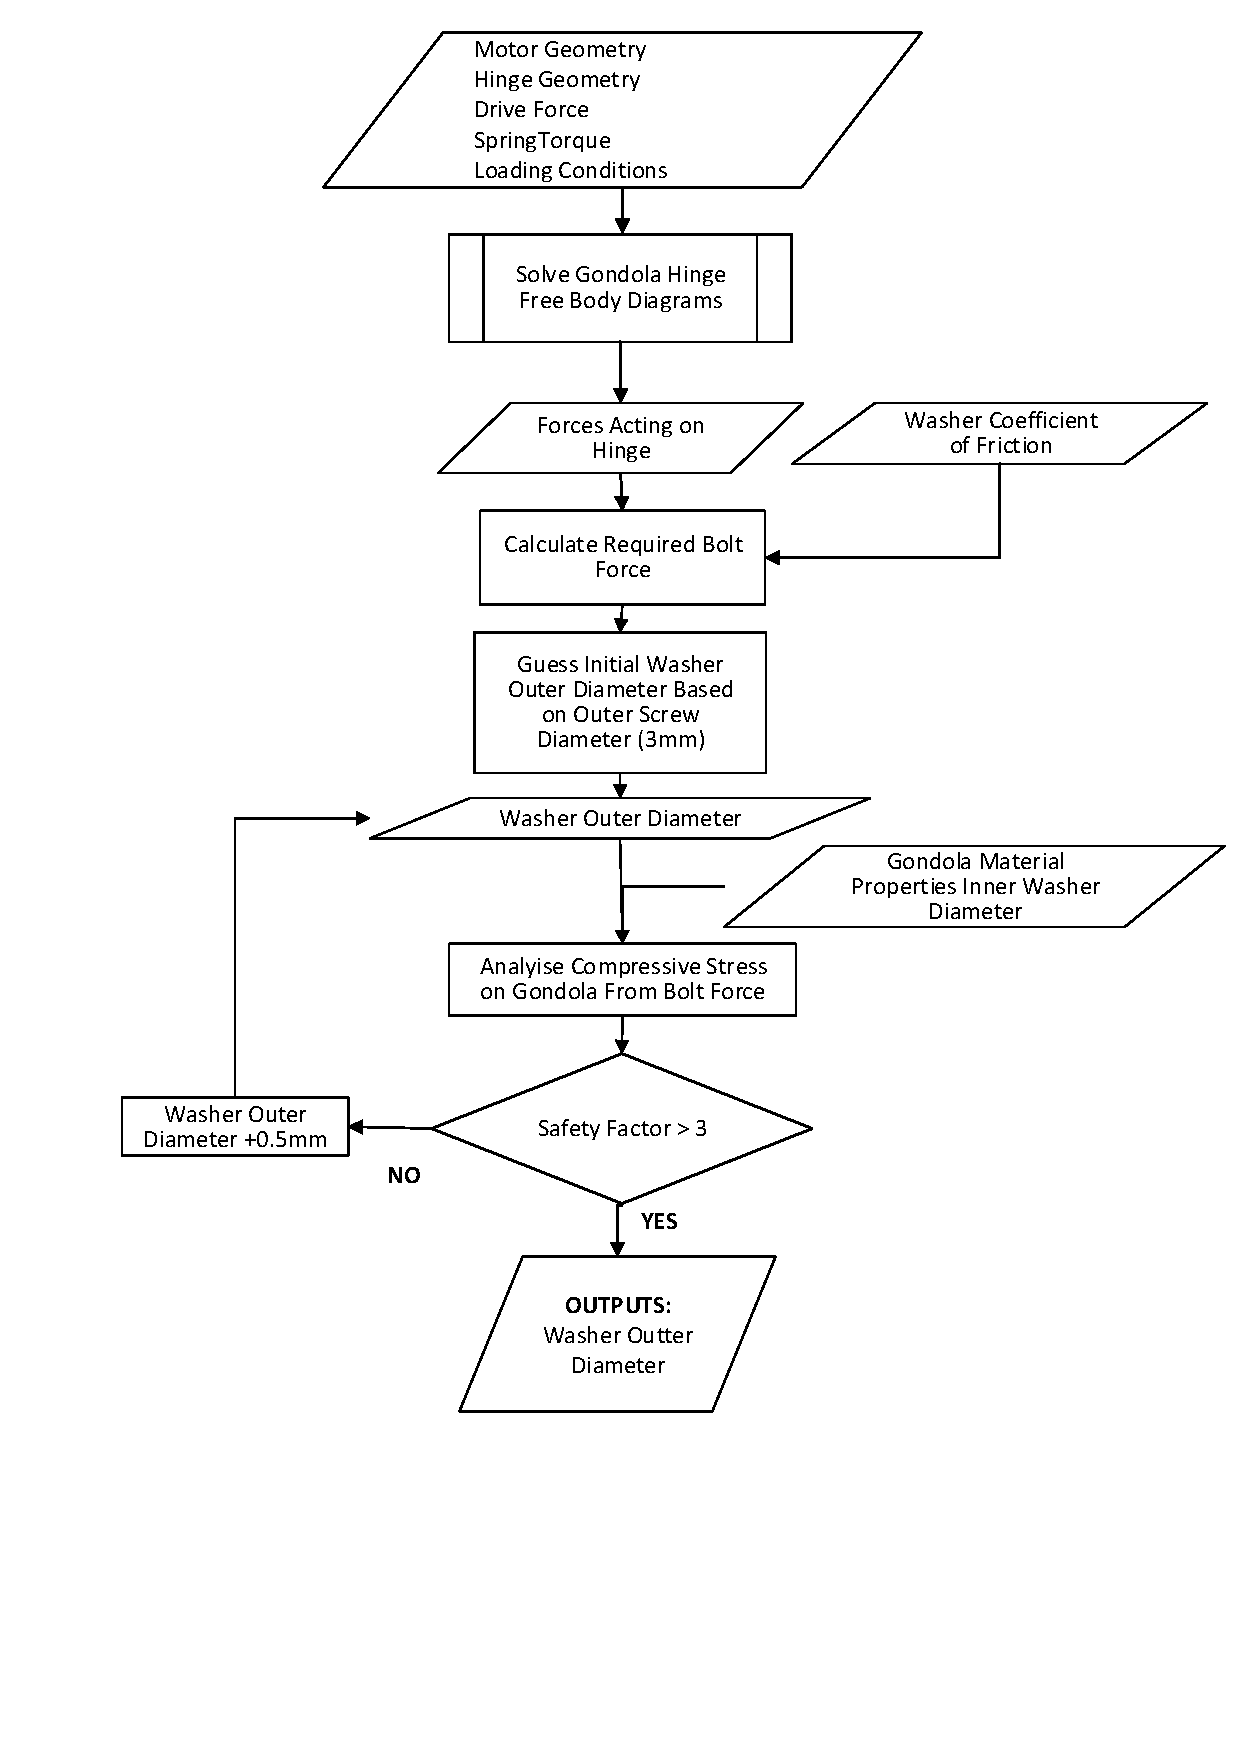
\includegraphics[width=.9\linewidth]{img/paramaterization/compressionBolt.pdf}
	\caption{Parametrization Outline for the Bolt Compression Force}
	\label{fig:boltCompressionParametrization}
\end{figure}

To fasten the metal hinge to the plastic gondola body, bolts will be used. The reason for this is that they use compression forces to join the two pieces, without requiring threading. Threading a screw into plastic would require female threads in 3D printed plastic, which is inherently bad design and would almost surely fail. \\

The main mode of failure for the bolts will not be for the bolt itself, as the forces involved in this design will surely be much less than the yield strength of any potential bolt used. The true concern is the plastic at the interface of the bolt being crushed. \\

The Bolt compression analysis is meant to ensure that for the Force $F_{bolt}$, generated by tightening the but and bolt attaching the hinge to the gondola, that the compressive stresses are withstand-able by the plastic. The required inputs for the analysis are geometry of the motor and hinge, the positions and size of the bolts used, the spring for ce from the hinge torsion spring and the drive force calculated from the motor torque. The analysis will output the required outer washer diameter that ensures a safety factor of 3 or greater. 
  
The analysis first computes the bolt tension required to resist the forces parallel to the surface of the hinge. The forces parallel to the bolt are shown in Figure \ref{fig:hingeForce}.
\begin{figure}[H]
	\centering
	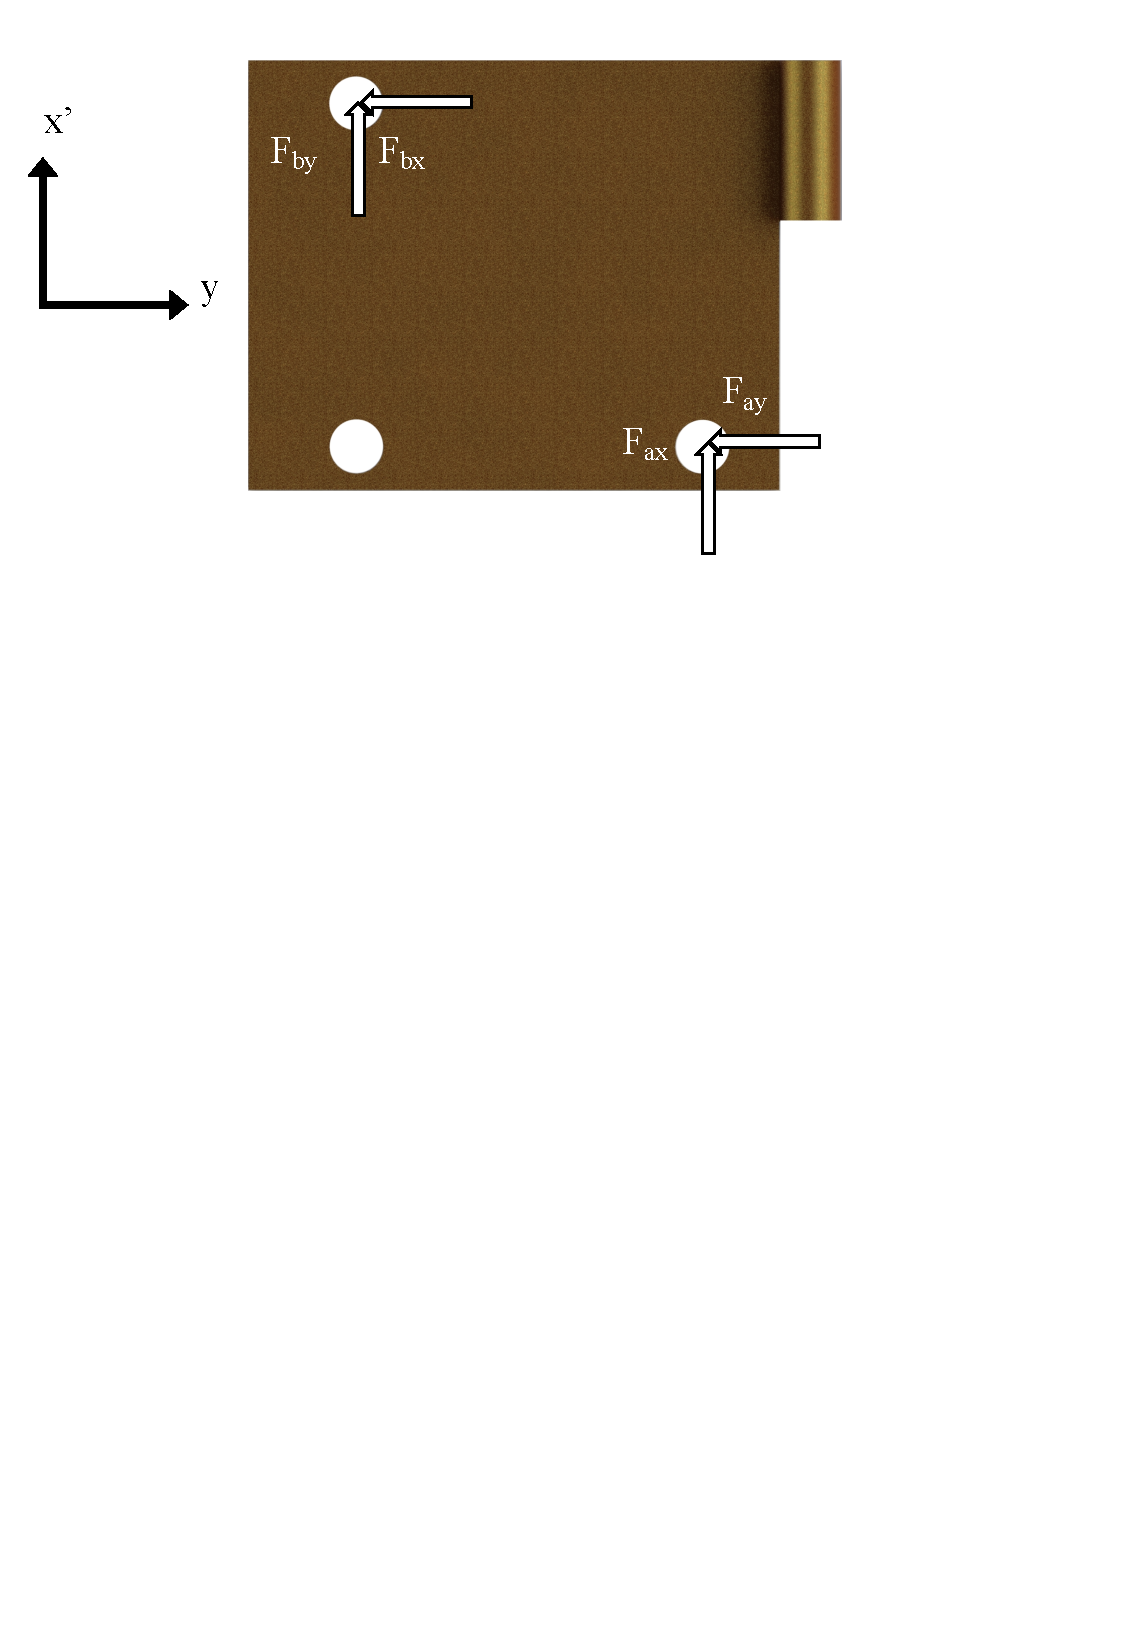
\includegraphics[width=1\textwidth]{img/gondola/hingeForces.pdf}
	\caption{Top View of Bottom Piece of Hinge}
	\label{fig:hingeForce}
\end{figure}
The resultant forces in the x'y plane are show below in Equation \ref{eqn:bshear}
\begin{displaymath}
\label{eqn:bshear}
F_{bshear} = \sqrt[]{F_{bx'}^2 + F_{by}^2}
\end{displaymath}

The only reaction resisting forces in the x'y plane will be the friction between the washer and the plastic. It is known that $F_f = \mu Normal Force$. In this case, the normal force is provided by the bolt tension $F_{bolt}$ shown in Figure \ref{fig:boltCrossSection}. 
\begin{figure}[H]
	\centering
	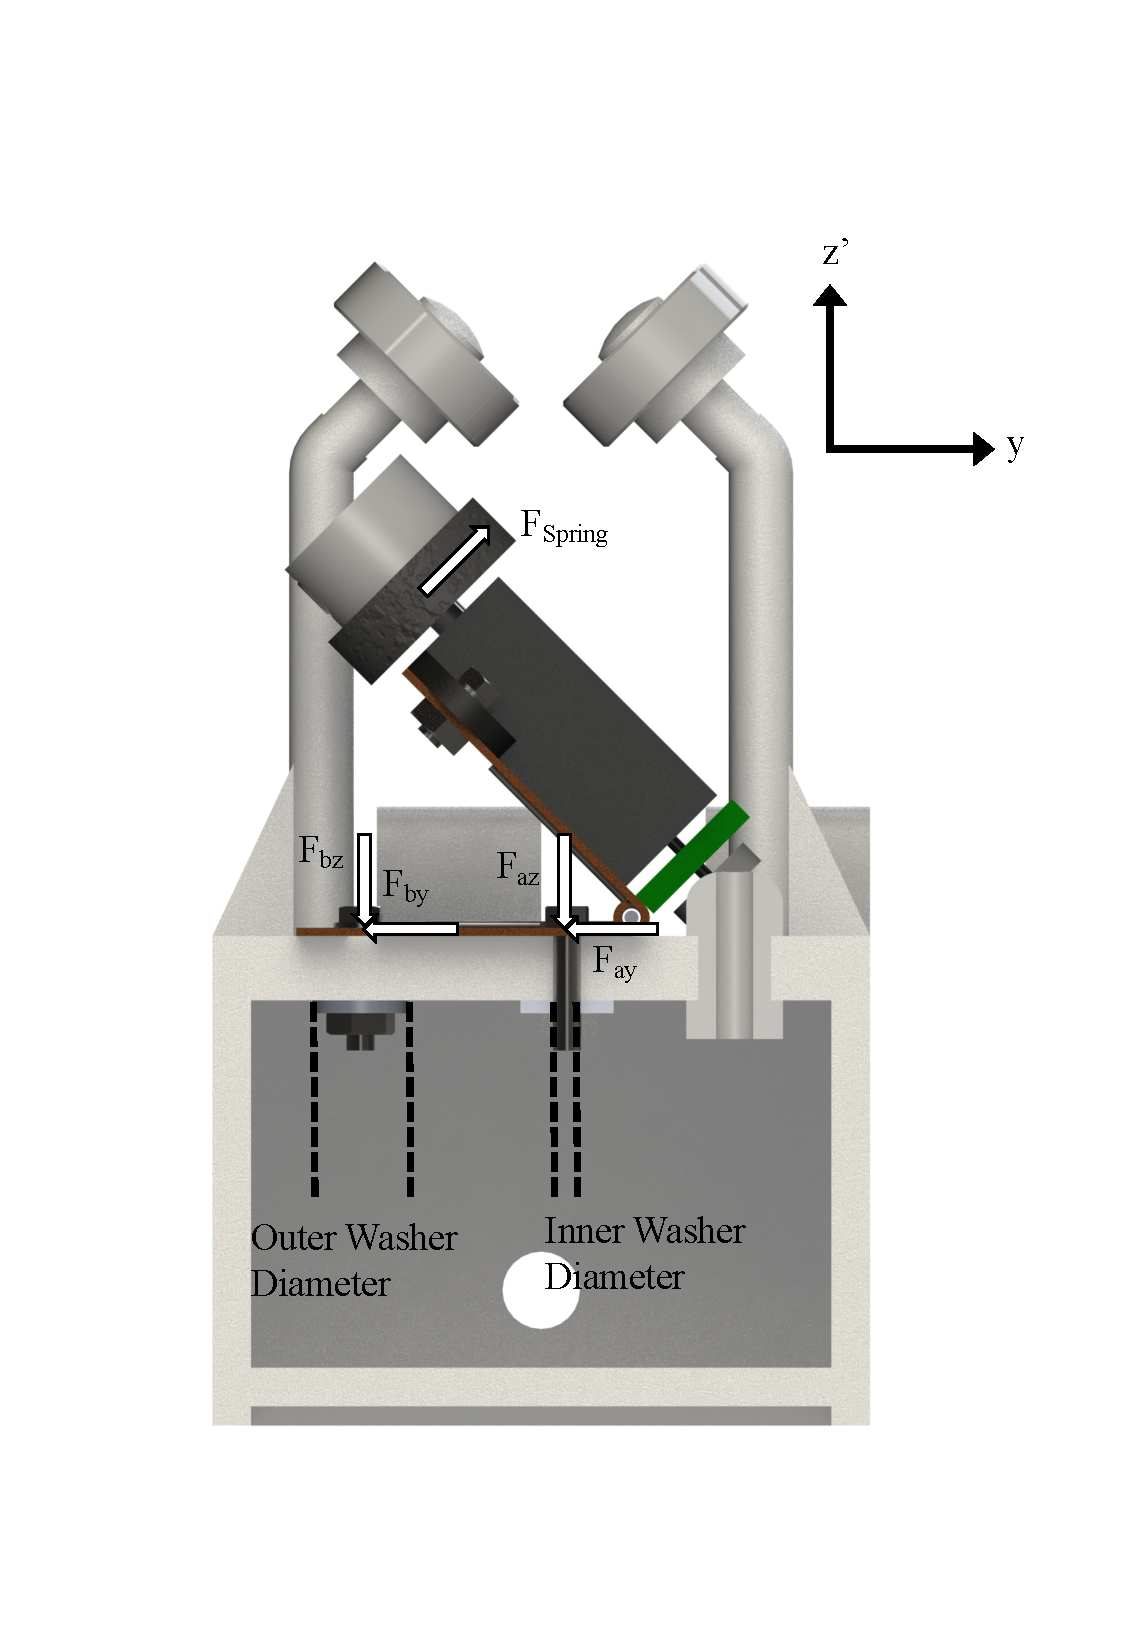
\includegraphics[width=0.9\textwidth]{img/gondola/boltCrossSection.pdf}
	\caption{Front View Cross Section of Gondola Hinge Bolts}
	\label{fig:boltCrossSection}
\end{figure}
This bolt tensions must be large enough to generate the required friction force as well as resist the forces acting on it in the z direction. Therefore the required bolt force to ensure no slipping due to shear forces is therefore
\begin{equation}
F_{bolt} = \dfrac{\sqrt[]{F_{bx}^2 + F_{by}^2}}{\mu} + F_{bz}
\end{equation}
$\mu $ is estimated as the coefficient of friction between polyethylene and steel, which is 0.2 \cite{Friction}. \\

Once $F_{bolt}$ is known, the compressive stress of the washer on the plastic gondola body can be determined. This is the critical design factor. If the compressive stress from the washer is too high it will crush the plastic underneath it.\\

The compressive yield strength ($S_{compressive}$) of Nylon 12  is found to be 6 MPa from the Appendix Datasheet \ref{3dProperties}. The compressive stress on the gondola by the washer is found to be 

\begin{align*}
\sigma _{washer} &= \dfrac{F_{bolt}}{A_{washer}}
\end{align*}
\begin{align}
\sigma _{washer} &= \dfrac{F_{bolt}}{\pi (r_o - r_i)^2}
\end{align}

\begin{equation}
\eta = \dfrac{S_{compressive}}{\sigma _{washer}}
\end{equation}

If the safety actor is less than 3 the analysis is reiterated with a larger washer outer radius. 
\end{document}